\documentclass[10pt]{report}
\usepackage[utf8]{inputenc}

\usepackage[a4paper,width=150mm,top=25mm,bottom=25mm]{geometry}
\usepackage[colorlinks = true,
            linkcolor = blue,
            urlcolor  = blue,
            citecolor = blue,
            anchorcolor = blue]{hyperref}
\usepackage{setspace}
\onehalfspacing

\usepackage{parskip}
\usepackage[document]{ragged2e}
\usepackage{hyperref}


\setlength{\marginparwidth}{2cm}\usepackage{todonotes}


\usepackage{xcolor}
\newcommand{\researchq}[1]{\large{\color{black} #1}}

\usepackage{titlesec}
\usepackage{lipsum}

% Referencing settings
\usepackage[backend=biber, style=apa, sorting=nyt]{biblatex}
\addbibresource{proposal/citations.bib}

\begin{document}

\title{EC331 - Research In Applied Economics \\ 
Project Outline
\vspace{150pt}

{Gender differences in sorting: Measurement and decomposition of productivity in academia} \\

\vspace{150pt}
}
\author{Milan Makany \\
u2048873}
\date{\today}

\maketitle\title{EC331 - Research In Applied Economics \\ 
Project Outline
\vspace{150pt}

{Gender differences in sorting: Measurement and decomposition of productivity in academia} \\

\vspace{150pt}
}
\author{Milan Makany \\
u2048873}
\date{\today}

\maketitle

\justify 
\section*{Project Outline}



\subsubsection*{Research Question}

Is there a gender differential in the sorting of academics?

\subsubsection*{Motivation and Objective}
The primary motivation of this research is to analyse gender differences in academia by providing insight into differences in sorting -- a discrepancy in high-productivity academics reaching high-productivity institutions. This is important for both societal and efficiency reasons, this research focusing on the latter. If the gap exists, it can potentially be explained by discrimination or an overall divergence in preferences.

%-- high-productivity women not reaching high-productivity departments --

%I aim to provide an insight into publication patterns and analyse the under representation of women in STEM fields.

In order to perform econometrics analysis I require a consistent cross-field measure of quality. This is vital as researchers have different publication patterns across fields and papers in journals of similar stature might have different impacts. I build on scientometric literature to construct a uniform measure of contribution using machine learning methods. To my knowledge no systematic analysis of this sort has been published.

Once I have a consistent measure of contribution, I deconstruct academic- and department-effects using an AKM model (\cite{Abowd1999}). I observe differences in the distribution of individual and department effects and analyse the sorting effect by field, and region.

\subsubsection*{Contribution}

This research has two contributions. First, I propose a method of comparing the quality of research across fields. This is a useful tool for grant and promotion committees along with academics looking to analyse science.
Second, the difference in sorting may help explain a part of the observed gender differences and highlight an inefficiency in how we organise science.

%the differences in network effects across gender could prove the presence of discrimination and explain the sorting of women into specific fields.

\subsection*{Methodology}
\label{sec:method}


\subsubsection*{Measure of Contribution}
\label{ssec:contrib}

\vspace{5pt}

\textit{I test multiple machine learning methods, this is a short summary of a selected few. For a more comprehensive review see \textcite[Chapter 19]{Kuhn2013}.}

\vspace{10pt}


I construct the metrics described in \textcite{Waltman2016} to obtain more than 100 measures of research quality and use machine learning to find the optimal weight assigned to each measure. For this to be feasible I construct a labeled database of academics and an outcome variable \textit{top\_institution}, equal to 1 if the academic is affiliated with an institution in the 95th percentile after the first ten years of their career and 0 otherwise.

I normalise all the measures to the range [0,1] using \autoref{eq:normalisation} and compute the vector of weights \(\vec{w}_f\) for each field by solving the optimisation problem in \autoref{eq:optimisation} using gradient descent. The only hyper-parameter of question for gradient descent is the learning rate which can be adjusted via trial and error.

\begin{equation}
    \label{eq:normalisation}
    contrib_i = \frac{contrib_i - min(contrib)}{max(contrib) - min(contrib)}
\end{equation}

\begin{equation}
    \label{eq:optimisation}
    \min_{w_m} \quad (top\_institution_i - \sum_m w_m score_{im})^2 \quad s.t. \quad \sum_{m} w_m = 1
\end{equation}

I also construct the vector of weights using a Neural Network that allows for more complex connection between the measures of contribution. \autoref{fig:nn_example} demonstrates how the weights in a hypothetical network look. The connections between the nodes (weights) are more visible if that connection is more important in explaining the outcome variable. The number and size of hidden layers along with other hyper-parameters can be optimised for the best results.


\begin{figure}[htbp]
    \centering
    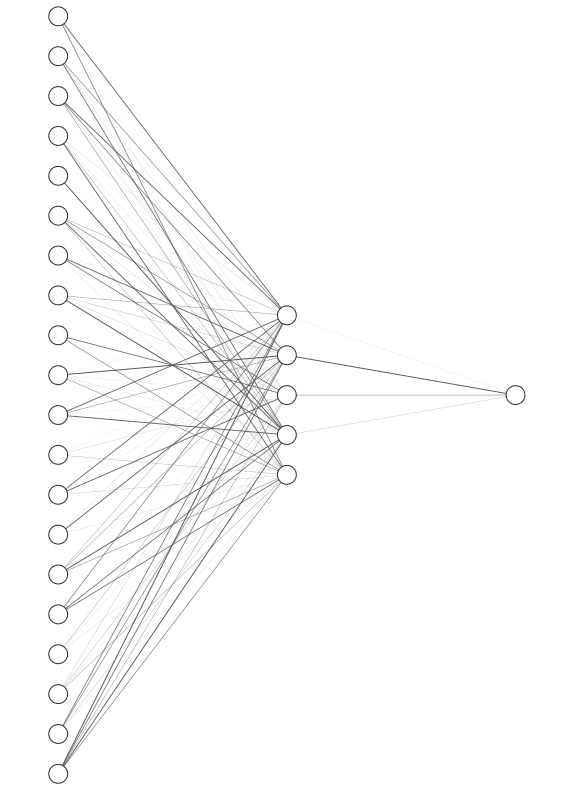
\includegraphics[scale=.4, angle =90]{proposal/nn.png}
    \caption{Example of a hypothetical neural network structure}
    \label{fig:nn_example}
\end{figure}


I verify this approach with promotion data from Italy and Spain \parencite[]{Bagues2017} by computing the same weights with a new outcome variable \textit{promoted}. If the obtained weights are significantly different, it is probable that the results are biased. In this case I will have to consider restricting the sample to certain fields which would reduce the external validity of the research.

\subsubsection*{Decomposition}

I decompose the individual and department effects using an AKM model in \autoref{eq:dec_model} \parencite[]{Abowd1999}.

\begin{equation}
    \label{eq:dec_model}
    contribution_{ikt} = \alpha_i + \delta_t + \varphi_{kt} + \varepsilon_{ikt}
\end{equation}

I estimate a simple two period model based on the specification proposed in \textcite{Bonhomme2019}, where \(\alpha_i\) captures the individual and \(\varphi_k\) captures the department effect. I define event time as the number of years since first publication as a professor. This is difficult to pin down as in some fields it is quite common to publish during the course of a PhD and pursue post-doctoral positions.

% , whereas in other fields such as economics it is quite uncommon (and outliers exists making this exercise even more difficult).

% observe one movement (or no movement) for each academic when they start their career after their PhD as associate professors (t=0) and after they get promoted to assistant professor (t=1).

In this two period model I first observe academics 5 years after their PhD working as Assistant Professors and then again 5 years later having worked as Associate Professors. (I have the data to estimate a more complex dynamic model, see \hyperref[sec:potential]{Potential For Further Research})

Sorting defined as \(cov(\alpha_i, \varphi_k)\) can be estimated separately for men and women. If the difference in sorting \(cov(\alpha_i, \varphi_k | female = 1) - cov(\alpha_i, \varphi_k | female = 0)\) is negative then I show that high-productivity women are less likely to make it to high-productivity departments.

The sign of the \(\varphi_{kt}\) coefficients is also of interest. The interpretation of these coefficients is somewhat complicated. Department effects are a function of conditions provided by the department: facilities, support, networks, etc. I estimate these department effects at different intervals to analyse trade-offs associated with institutions providing different levels of support and assigning different amounts of administrative and teaching duty to academics in certain stages of their career.

\subsubsection*{Identification}

The first condition for identification is to have enough variation in the data to estimate the fixed effects. I expect a large variance in publication patterns and quality, hence too little heterogeneity is not likely to be an issue.

The second requirement is a sufficient number of movers. It is reasonable to assume that the mobility in academia is sufficient for estimation, however this can be only verified by observing the data. 

Third, institutions have to be connected to each other via movers \parencite{Abowd2002}. If this fails using university-academic level data, I will group institutions with a k-means clustering algorithm \parencite{Bonhomme2019} or analyse a limited set of institutions and academics.

The fixed effects model also relies on the assumption of random timing in movements. This assumption is very strong and likely to be violated as moves in academia are usually associated with promotions and are endogenous. I will have to analyse the reasons for moving and ease this assumption.

\subsubsection*{\hyperref[ssec:data]{Data Description}}

\newpage
\section*{Literature Review}
\label{sec:lit}

How do we conduct science? We must understand the organisation of discovery and the diffusion of knowledge. \textcite{Stephan2012} provides a detailed description of the scientific research process. They emphasize the variance in the process of production and collaboration across fields. The two key components of research are clearly defined: individual knowledge, persistence and ability (individual-effect captured by \(\alpha_i\)) and environment, facilities, and networks (department-effect captured by \(\varphi_k\)). The AKM setup is well-suited for the analysis of production in science since the two main components of productivity are captured in the model. A possible extension of this research is to further decompose department effects and analyse what factors of production are most important in stages of an academic's career.

\textcite{Waldinger2012} shows that faculty quality has long-term effects on the productivity of PhD students and furthermore, high-quality scientists attract talent and funding (\cite{Waldinger2016}; \cite{Azoulay2010}). From an efficiency perspective this implies that it is beneficial to match high-productivity academics and that high-productivity departments provide the environment that allows for science to augment.

It is widely documented that there are persistent gender differences in science (\cite{Gasser2014}; \cite{Lariviere2013}; \cite{Iaria2022}). These inequalities transmit through multiple channels, one of which is the inefficiency they create. If high-productivity women are less likely to match to high-productivity environments and hence other high-productivity academics we do not utilise their potential and lose out on crucial peer effects. \textcite{Ganguli2015} shows that studies published before moving to a \textit{better} department receive more attention after the move, implying that if a gap in sorting exists then women's publications are systematically under-utilised.

The importance of understanding gender dynamics in sorting is clear. In order to analyse it I use an AKM approach adopted by \textcite{Card2016} to study the gender wage gap. The methodology they use to identify the gender differences can be perfectly applied for answering my research question. The novelty of my research is that the individual effects \(\alpha_i\) can be interpreted in a more straight-forward manner since scientific productivity is public and directly observed. If a difference in sorting exists how do we interpret it? Is it a simple difference in preferences or are women systematically discriminated against? To answer this question is very ambitious and to do so I would need to infer preferences (for example like \cite{Sorkin2017}) or construct some measure of discrimination.

To perform the decomposition I first have to create a metric that measures contribution consistently across fields. There is an extensive discussion in the Scientometrics literature about comparing the quality of publications by different authors in different fields.
\textcite{Radicchi2008} shows that citation patterns vary greatly across fields and claims that using a scaled measure of citations (\autoref{eq:radicchi2008}) produces a universally comparable metric across disciplines.

\begin{equation}
    \label{eq:radicchi2008}
    c_f = \frac{c_i}{\bar{c}}
\end{equation}

Their claim is investigated by \textcite{Waltman2012} using a larger sample of fields and publications. They only find circumstantial evidence to support the conclusion that this scaled metric allows for valid comparison across fields. Unfortunately, I do not find the results convincing and since I heavily rely on cross-field comparability, I use machine learning techniques outlined in \hyperref[sec:method]{Methodology}.

\printbibliography

\newpage
\section*{Appendix}
\label{sec:appendix}

\subsection*{Potential For Further Research}
\label{sec:potential}

\subsubsection*{Model Extensions}

The network effects at institutions are of key interest. I estimate the model in \autoref{eq:dec_model2} where I control for the network of individuals. Close network defined as co-authors and broad network as colleagues. Note that close network has the subscript \textit{i} because it depends on the specific person but the broad network depends on the department (excluding academic i) hence the \textit{k} subscript.

\begin{equation}
    \label{eq:dec_model2}
    contribution_{ikt} = \alpha_i + \delta_t + \varphi_{kt} + net\_close_{it} + net\_broad_{ikt} + \varepsilon_{ikt}
\end{equation}

These network effects might be vital to explaining the difference in sorting. If women benefit disproportionately little from their broad network (colleagues) they have less incentives to sort into high-productivity departments and rather focus their efforts on building their close network. 

This exercise is quite feasible as \textcite{Bonhomme2019} provide the methodology for estimating more complex dynamic models and could spur more research questions.


\subsubsection*{Evolution of Fields}
\label{ssec:evfield}
Having found the best method for constructing a field-consistent measure of contribution I can use the algorithm to obtain the appropriate weights for fields throughout time (recalculating the weights each decade or so). I expect that more recently established (young) fields such as economics place a higher weight on the biggest contribution (best paper published by an author), while older fields might place higher weights on the number of publications.

Tracking the evolution of fields this way might provide insight for new academics on what to focus on at the start of their career if they want to be successful in the future.

\subsubsection*{Inequality of Opportunity}

In a similar manner as in \hyperref[ssec:evfield]{Evolution of Fields} I can also track the probability of making it to a top institution, given the academic is a top-productivity individual (based on the decomposition).

\begin{equation}
    \label{eq:prob_gender}
    P(Top\_Inst | Top\_Academic, Female = 1) - P(Top\_Inst | Top\_Academic, Female = 0)
\end{equation}

I define the gender gap in opportunity in \autoref{eq:prob_gender}. This can be estimated for multiple time periods, where time can be defined in absolute terms or the maturity of a field (time since first journals established). The same analysis can be done using the AKM model in \autoref{eq:dec_model} to track the dynamics of sorting. This descriptive analysis could be useful in understanding how gender dynamics evolve in academia across and within fields.


\subsubsection*{Understanding Research}

This study's primary goal is to provide insight into the \textit{machinery} of academia. However, in the process of constructing measures of contribution I approach the issue from a purely statistical perspective. I find it important to understand why certain metrics carry more weight than others; is this an accurate reflection of how science contributes to society or rather a reflection of how academics judge each other in the process of promotions. There is a short review of the difference between bibliometrics and scientometrics in the \hyperref[sec:lit]{Literature Review} and the \hyperref[ssec:bibvscient]{Appendix}.

\subsubsection*{Rankings}
\label{ssec:rankings}
Comparing the department fixed effects to the already existing rankings is an interesting exercise. This tool could be useful for academics when facing a decision of where to move. Based on the predictions of this model they would be best off going to a place with a very high estimated department fixed effect \(\varphi_k\).

\subsection*{Data Description}
\label{ssec:data}

I use publication data from OpenAlex, "an index of hundreds of millions of interconnected entities across the global research system" \parencite[]{Priem2022}. They provide an open-access database of publications, author affiliations, journals, the number of citations since publication (in some cases even the citations of the working paper, before publication) and the works cited by the authors.

\centering\hyperlink{https://docs.openalex.org/about-the-data}{The official documentation of the objects in OpenAlex}

\begin{figure}[htbp]
    \centering
    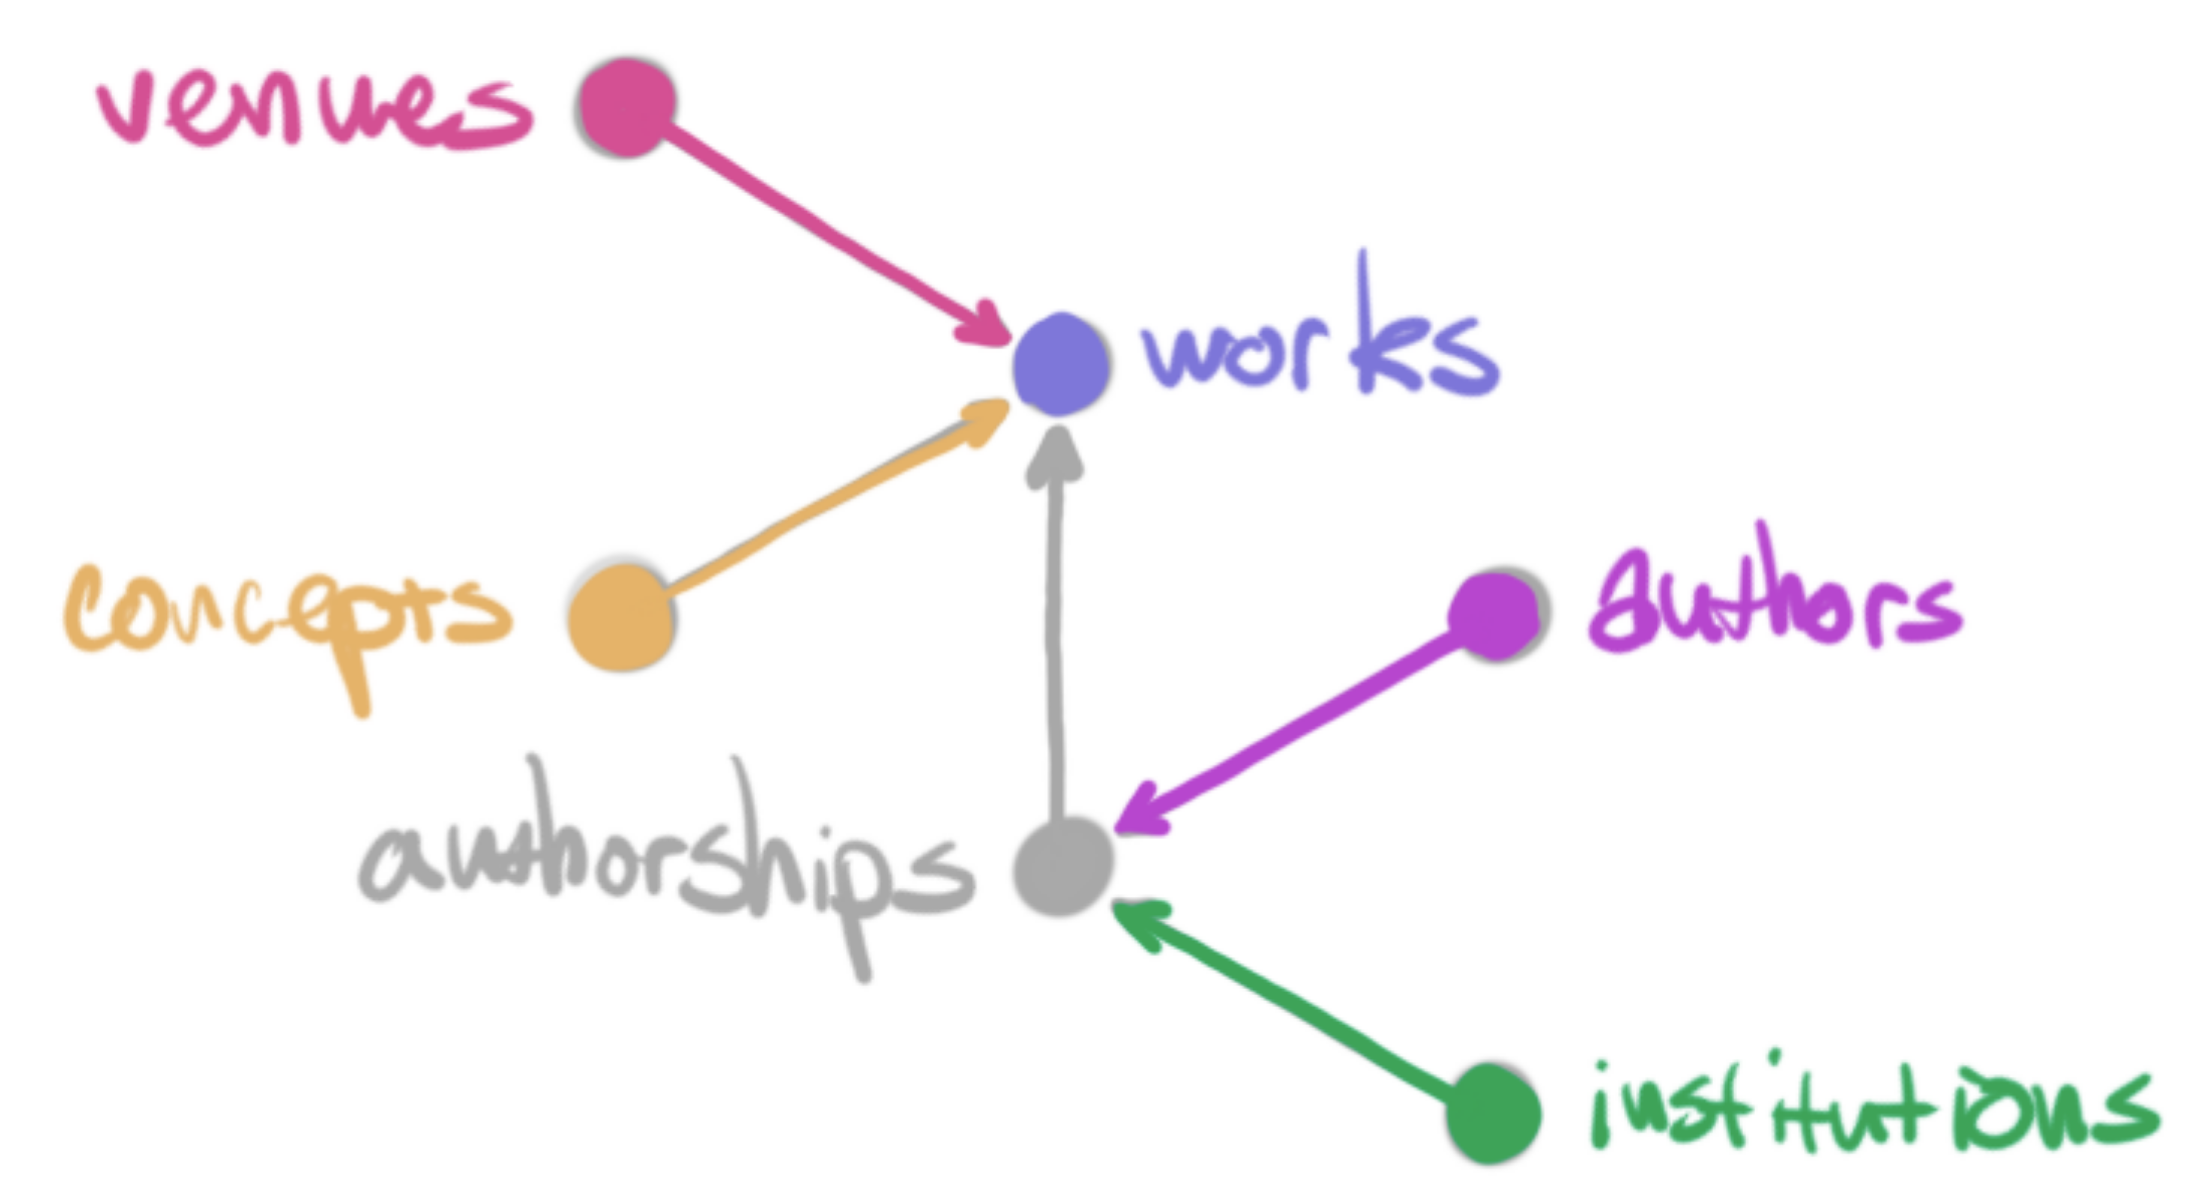
\includegraphics[scale=.1]{proposal/openalex.png}
    \caption{Connection of OpenAlex Objects}
    \label{fig:openalex}
\end{figure}

\justify OpenAlex has data of 6 different types shown in \autoref{fig:openalex}. The primary object of interest for my research is Works. This object contains data from all other objects and has references to the other objects in case I need some additional data not contained in Works.
The data is stored in JSON format (equivalent of dictionaries in Python), a list of key-value pairs.
Samples of objects can be found in \autoref{tab:openalex}.

\vspace{10pt}

\begin{table}[htbp]
    \centering
    \begin{tabular}{c|c}
         Authors & \hyperlink{https://api.openalex.org/people/A2056708386}{https://api.openalex.org/people/A2056708386} \\
         Works &  \hyperlink{https://api.openalex.org/works/W3121763541}{https://api.openalex.org/works/W3121763541} \\
         Venues & \hyperlink{https://api.openalex.org/journals/V203860005}{https://api.openalex.org/journals/V203860005} \\
         Institutions & \hyperlink{https://api.openalex.org/institutions/I39555362}{https://api.openalex.org/institutions/I39555362} \\
         
    \end{tabular}
    \caption{OpenAlex Objects}
    \label{tab:openalex}
\end{table}

\subsection*{Data Collection and Extraction}

There are multiple methods for extracting data from OpenAlex. They provide a public API with a rate limit of 10 requests per second and they provide snapshot saves of the entire compressed database from AWS.

I copied a snapshot of the database (323 GB) onto an external SSD and then to the University's Scientific Computing Research Technology Platform (SCRTP) cluster computer. From this compressed database I extract the data using Python and then process it using either Python or Stata.

If the snapshot turns out to be incomplete or unable to process the API is the second best option. Using Python I can send a series of HTTP requests to download publication data. This process is more time consuming, however the time allocated to programming would be reduced.

\subsection*{Bibliometrics v Scientometrics}
\label{ssec:bibvscient}

Bibliometrics in general is more about understanding what quality is rather than simply looking for ways to measure it. Scientometrics literature focuses more on creating metrics which measure the academic's contribution based on observable statistics.


Example of a bibliometric approach in \textcite[p. 151]{Moed2006}
\begin{quote}
\textit{First, one should collect documents containing statements
of scholars in the field under study on how assessment of research
performance should be conducted, and, of course, on how it should not be
conducted. Earlier reports of peer review committees evaluating scholars in
the field constitute a fruitful basis for such an inventory. The bibliometric
investigator should identify the main aspects of research quality involved,
issues that were raised, problems that remained unsolved, operationalisations
that were applied or rejected. Secondly, scholars from the field should be
involved in all stages of the study. They should be stimulated to propose or
develop – even preliminary – classification systems, and to structure their
own research output accordingly.}

\end{quote}

\vspace{10pt}

Example of a scientometric approach in \textcite[p. 20]{Waltman2016}

\begin{quote}
\textit{In the calculation of citation impact indicators, citations are sometimes taken into
account only within a specific time period after the appearance of a publication, the
so-called citation window. Adopting a certain citation window may cause both
publications and citations to be excluded from the calculation of citation impact
indicators. For instance, suppose we require publications to have a citation window of
at least five years. For recent publications it is not possible to have a five-year citation
window, and therefore this requirement implies that recent publications cannot be
included in the calculation of citation impact indicators.}

\end{quote}


In general I find the bibliometric approach more appealing as it aims to provide a deeper understanding of research and how to define contribution, however for the goals of this project the scientometric approach is more important. A natural extension of this study is to understand why certain scientometric indicators are more important than others and this is where methods from the bibliometric approach should be adopted.


\end{document}
